\documentclass[tikz,border=8pt]{standalone}
\usepackage{amsmath,amssymb}
\usetikzlibrary{arrows.meta,calc,patterns}

\begin{document}
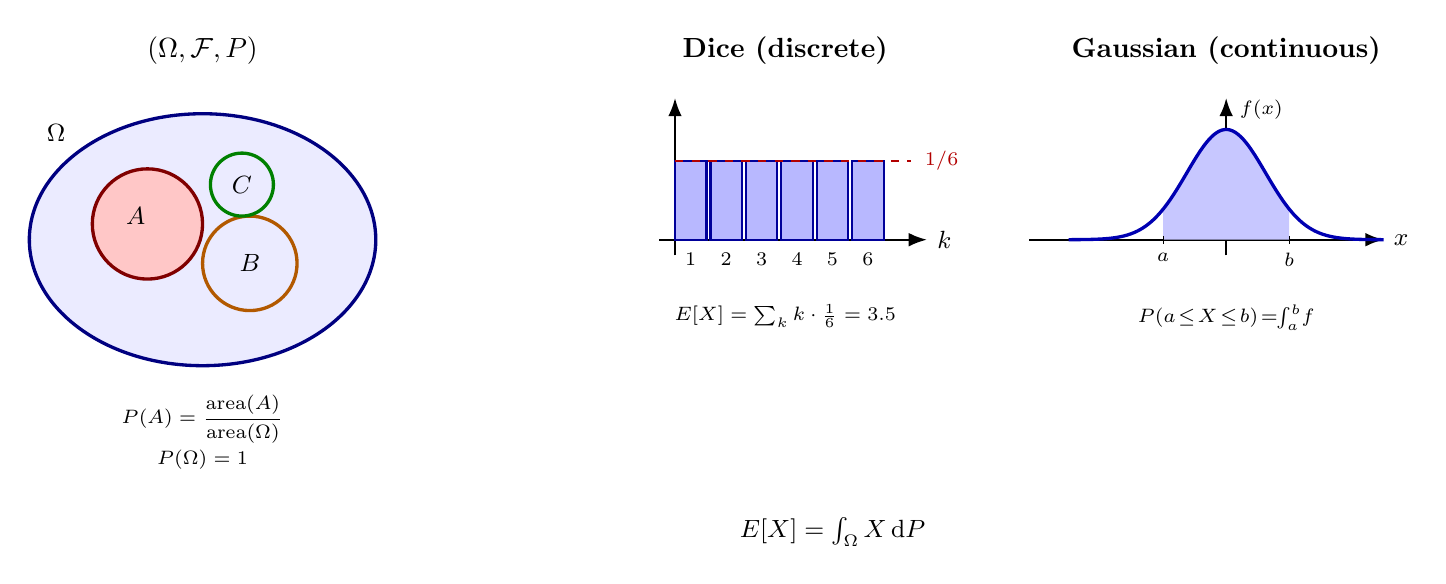
\begin{tikzpicture}[>=Latex]

  % LEFT: Ω with events
  \begin{scope}[xshift=0cm]
    \node[font=\bfseries] at (0, 2.4) {$(\Omega, \mathcal F, P)$};
    \draw[very thick, blue!50!black, fill=blue!8] (0, 0) ellipse (2.2 and 1.6);
    \node[font=\small, anchor=west] at (-2.1, 1.35) {$\Omega$};

    \filldraw[red!50!black, fill=red!22, very thick] (-0.7, 0.2) circle (0.7);
    \node[font=\small] at (-0.85, 0.3) {$A$};

    \draw[orange!70!black, very thick] (0.6, -0.3) circle (0.6);
    \node[font=\small] at (0.6, -0.3) {$B$};

    \draw[green!50!black, very thick] (0.5, 0.7) circle (0.4);
    \node[font=\small] at (0.5, 0.7) {$C$};

    \node[font=\scriptsize, anchor=north, align=center] at (0, -1.85) {$P(A)=\dfrac{\text{area}(A)}{\text{area}(\Omega)}$};
    \node[font=\scriptsize, anchor=north] at (0, -2.55) {$P(\Omega)=1$};
  \end{scope}

  % MIDDLE: dice histogram
  \begin{scope}[xshift=6cm]
    \node[font=\bfseries] at (1.4, 2.4) {Dice (discrete)};
    \draw[->, thick] (-0.2, 0) -- (3.2, 0) node[right, font=\small]{$k$};
    \draw[->, thick] (0, -0.2) -- (0, 1.8);

    \foreach \k in {1,...,6}{
      \pgfmathsetmacro{\bx}{(\k-1)*0.45}
      \filldraw[blue!28, draw=blue!60!black, thick] (\bx, 0) rectangle ({\bx+0.4}, 1.0);
      \node[font=\scriptsize, anchor=north] at ({\bx+0.2}, -0.05) {\k};
    }
    \draw[red!70!black, thick, dashed] (0, 1.0) -- (3.0, 1.0);
    \node[font=\scriptsize, anchor=west, red!70!black] at (3.05, 1.0) {$1/6$};

    \node[font=\scriptsize, anchor=north] at (1.4, -0.7) {$E[X]=\sum_k k\cdot\tfrac{1}{6}=3.5$};
  \end{scope}

  % RIGHT: continuous Gaussian
  \begin{scope}[xshift=11.5cm]
    \node[font=\bfseries] at (1.5, 2.4) {Gaussian (continuous)};

    \draw[->, thick] (-1.0, 0) -- (3.5, 0) node[right, font=\small]{$x$};
    \draw[->, thick] (1.5, -0.2) -- (1.5, 1.8);

    \fill[blue!22] plot[smooth, samples=60, domain=0.7:2.3] (\x, {1.4*exp(-(\x-1.5)*(\x-1.5)/0.5)}) -- (2.3, 0) -- (0.7, 0) -- cycle;

    \draw[blue!70!black, very thick, smooth, samples=120, domain=-0.5:3.5]
      plot(\x, {1.4*exp(-(\x-1.5)*(\x-1.5)/0.5)});

    \draw[thin] (0.7, 0.05) -- (0.7, -0.05) node[below, font=\scriptsize]{$a$};
    \draw[thin] (2.3, 0.05) -- (2.3, -0.05) node[below, font=\scriptsize]{$b$};

    \node[font=\scriptsize, anchor=south west] at (1.55, 1.4) {$f(x)$};
    \node[font=\scriptsize, anchor=north, align=center] at (1.5, -0.7) {$P(a\!\le\! X\!\le\! b)\!=\!\!\int_a^b\! f$};
  \end{scope}

  % Bottom unifying formula
  \node[font=\small, anchor=north] at (8.0, -3.4) {$E[X]=\int_\Omega X\,\mathrm dP$};
\end{tikzpicture}
\end{document}
